\documentclass[11pt]{article}

\usepackage[utf8]{inputenc}
\usepackage[T1]{fontenc}
\usepackage{lmodern}
\usepackage[a4paper,margin=1in]{geometry}
\usepackage{microtype}
\usepackage{amsmath,amssymb}
\usepackage{graphicx}
\usepackage{booktabs}
\usepackage{multirow}
\usepackage{array}
\usepackage{xcolor}
\usepackage{authblk}
\usepackage[numbers,sort&compress]{natbib}
\usepackage{tikz}
\usetikzlibrary{positioning,arrows.meta,fit,backgrounds}
\usepackage[hidelinks]{hyperref}
\usepackage{xurl}
\usepackage[section]{placeins}
\usepackage[capitalise,noabbrev]{cleveref}

\graphicspath{{figures/}}
\newcommand{\cls}{\texttt{cls}}
\newcommand{\mt}{\texttt{mt}}
\newcommand{\todo}[1]{\textcolor{red}{[TODO: #1]}}
\renewcommand\Affilfont{\small}

\title{A Controlled, Pre-specified Evaluation of Multi-task Learning\\ for Utility-Pole Lean Assessment}

\author[1]{Mahdi Mohammadiha}
\author[1,*]{Mahdi Bahaghighat}
\affil[1]{Department of Computer Engineering, Imam Khomeini International University, Qazvin, Iran}
\affil[*]{Corresponding author: \texttt{bahaghighat@eng.ikiu.ac.ir}}
\date{}

\begin{document}

\maketitle

\begin{abstract}
Automated assessment of leaning utility poles from smartphone images can support the inspection of power
distribution networks, and pole-axis keypoints are an obvious source of extra supervision for this task.
We study whether such geometric supervision improves image-level lean classification (Leaned / Straight /
Rejected) on the public PD-Defect dataset, using fully fine-tuned DINOv2 vision transformers. All comparisons
use equal-budget hyper-parameter tuning on validation data, several training seeds, a single evaluation on
the official test split, and paired statistics (bootstrap confidence intervals, McNemar tests with Holm
correction). Every follow-up hypothesis was specified in a time-stamped version-controlled repository before it was run.
First, we show that the dataset's keypoint split contains 125 of the 227 classification-test images, so
combining the two tasks naively leaks test data; we give a leakage-free protocol. Second, ground-truth axis
angles reveal that the binary lean label follows an implicit threshold of about $3^\circ$ (a single
threshold reproduces 91.6\% of the test labels), not the $10^\circ$ rule used by the dataset authors, and that
residual errors concentrate in the ambiguous 2--$6^\circ$ band. Third, after tuning, an auxiliary keypoint
loss does not change classification quality on either backbone ($+1.2$ and $-1.3$ Macro-F1 points, both
confidence intervals containing zero), nor with 10--50\% of the training data, nor with stronger photometric
augmentation. Angle-aware soft targets improve calibration (test NLL $0.58 \rightarrow 0.48$), but controls
with shuffled angles or uniform smoothing of the same mass do equally well, so the gain comes from target
smoothing rather than from geometry. Finally, saliency and occlusion analyses show that every model relies causally on the pole
(blurring it flips about half of the predictions) and also on its surroundings; keypoint supervision increases
this reliance only for DINOv2 with registers, and the backbone whose attention is most pole-focused is the less
accurate one. The joint model still predicts the pole axis (mean angle error $0.97^\circ$) at no
cost in accuracy.
\end{abstract}

\noindent\textbf{Keywords:} power distribution inspection; utility pole; multi-task learning; vision transformer;
label smoothing; calibration; explainability; data leakage

% =====================================================================================================
\section{Introduction}
\label{sec:intro}

Leaning utility poles are a common defect in power distribution networks. A pole that leans can bring
conductors closer to the ground, strain its stays and fittings, and eventually fail. Utilities therefore
inspect poles regularly, and much of this work is now supported by images taken by field staff with
smartphones or by drones. Automating the first screening step, deciding from an image whether a pole is
leaning, could reduce the inspection workload, and recent systems address this and related tasks from
smartphone, UAV and other monocular images
\citep{masabathula2026smartphone,luo2026pole,wang2024leaning}.

Lean is a geometric property. It is natural to expect that a model which is taught where the pole axis is
should also be better at deciding whether the pole leans. The recently released PD-Defect dataset
\citep{pddefect_data} makes this question testable: its \texttt{pole\_lean\_assessment} subset provides
image-level lean labels (Leaned / Straight / Rejected) and, separately, two keypoints per pole that mark the
bottom and the top of its axis. The dataset authors use the keypoints in a separate pose model whose predicted
angle is thresholded at $10^\circ$ in a supplementary rule \citep{masabathula2026smartphone}, while the
image-level baseline on the dataset card is a DINOv3 ViT-B/16 classifier \citep{simeoni2025dinov3}.

In this paper we ask whether the keypoints help the \emph{classifier}. We train a single vision transformer
with a classification head and an auxiliary keypoint head (multi-task learning, \citealp{caruana1997multitask})
and compare it with the same network trained for classification only. Because the test set is small (227
images) and fine-tuning large transformers is noisy, a naive comparison can easily produce a spurious
``improvement''. We therefore treat the study as a controlled evaluation. Both variants receive the same
hyper-parameter search budget on validation data, every configuration is trained with several seeds, the test
split is evaluated once, and differences are reported with paired bootstrap confidence intervals and exact
McNemar tests with Holm correction. Each follow-up hypothesis, with its prediction and decision rule, was
written to a time-stamped version-controlled repository before the corresponding runs, and every outcome is reported.

Beyond the main comparison, we look at what limits accuracy on this dataset, whether the keypoint geometry
helps in other ways (with less training data, with stronger augmentation, or as angle-aware training
targets), and whether keypoint supervision changes where the classifier looks.

The answers form a consistent picture. We first show that the keypoint split of PD-Defect contains 125 of the
227 classification-test images, so that combining the two tasks naively leaks test data, and we use a
leakage-free protocol throughout (\cref{sec:leakage}). Ground-truth axis angles then reveal that the binary
label follows an implicit threshold of about $3^\circ$, that current models are within about one point of the
resulting label-consistency ceiling on Leaned vs.\ Straight, and that errors concentrate in the 2--$6^\circ$
band (\cref{sec:labels,sec:errors}). After equal-budget tuning, keypoint supervision does not change Macro-F1
on DINOv2 or DINOv2 with registers, nor with less training data or stronger photometric augmentation
(\cref{sec:main,sec:h1,sec:h3}). Angle-aware soft targets improve calibration, but controls with shuffled
angles and with uniform smoothing show that this gain comes from smoothing rather than from the angle
(\cref{sec:h2}). Finally, saliency and occlusion analyses show that all models rely on the pole and on its
surroundings, that keypoint supervision increases the reliance on the pole only for one of the two backbones,
and that better pole-focused attention does not go with higher accuracy (\cref{sec:xai}).

% =====================================================================================================
\section{Related work}
\label{sec:related}

Pole inclination has been estimated from UAV images with a detector or segmentation network followed by
geometric angle estimation, such as Hough-transform line detection or PCA-based line fitting \citep{alam2020resilience,luo2026pole}, from
street-level imagery with a detection transformer and a segmentation head whose masks are used for line fitting
\citep{dickinson2025pole}, from a segmented image combined with a 3D point cloud \citep{chen2023inclination},
and from monocular images with training-free geometric reasoning
\citep{wang2024leaning,wang2026overheadwires}. The PD-Defect authors deploy a smartphone-based pipeline in
which a YOLO12m detector labels poles as leaned or straight and a separate YOLO12m pose model predicts the axis
keypoints, whose angle is compared with a $10^\circ$ threshold in a supplementary rule
\citep{masabathula2026smartphone}. In these systems, the pole angle comes from a separate geometric or
pose-estimation step, not from a network trained jointly with the lean classifier. We instead study joint
training of one network, and measure what the geometric supervision does to the classifier.
\citet{wang2026overheadwires} extend their earlier method to poles together with overhead wires: from a single
uncalibrated image they extract line segments and vanishing points, group pairs of segments by position and
orientation into candidate pole faces and wires, and reconstruct both, with their tilt angles, in a relative
3D scene without any training. They compare the estimated poles with ground-truth annotations on leaning-pole
datasets, using deep segmentation networks as baselines, and do not address image-level lean classification;
their model is hand-designed geometry, whereas ours is trained jointly for classification and keypoints and
evaluated in controlled, pre-specified experiments.

Auxiliary tasks can act as an inductive bias and a regulariser \citep{caruana1997multitask,ruder2017overview};
keypoints can be regressed directly from deep features \citep{toshev2014deeppose}, and our
keypoint head uses learned queries that cross-attend to patch tokens, in the spirit of
DETR \citep{carion2020detr}. Whether such auxiliary supervision helps the main task is known to depend on the
task pair and on tuning, which is why we tune both variants with the same budget.

As backbones, DINOv2 \citep{oquab2024dinov2} provides strong self-supervised ViT features \citep{dosovitskiy2021vit}.
\citet{darcet2024registers} showed that large ViTs create high-norm ``artifact'' tokens in background
regions, and that extra register tokens remove them; we compare both variants and use this finding in the
explainability analysis.

Label smoothing \citep{szegedy2016inception} improves calibration and changes the geometry of the learned
representation \citep{muller2019labelsmoothing}; modern networks are often over-confident
\citep{guo2017calibration}. Soft labels derived from human disagreement can improve robustness
\citep{peterson2019human}, and label errors can be found even in widely used benchmark datasets
\citep{northcutt2021confident}.
Our angle-aware targets are a measurement-based form of soft labelling, and we compare them with plain
smoothing of the same mass.

For transformers, gradient-based maps such as Grad-CAM \citep{selvaraju2017gradcam}, raw or rolled-out attention
\citep{abnar2020attention} and relevance propagation \citep{chefer2021transformer} are common, but saliency
maps can be insensitive to the model \citep{adebayo2018sanity}. We therefore combine them with an occlusion test, which
measures how the prediction changes when a region is removed, and we evaluate the maps themselves by a deletion
test and a sanity check, in addition to the energy inside a ground-truth box and the pointing game
\citep{zhang2018excitation}.

Finally, leakage between training and test data is a frequent source of over-optimistic results
\citep{kapoor2023leakage}. Variance from data sampling, data order and initialisation is of the same order as many reported
improvements \citep{bouthillier2021variance}, and McNemar's test is an acceptable paired test for classifiers
trained once and compared on one test set \citep{dietterich1998tests}. Pre-registration of hypotheses is advocated in other sciences as a guard
against analytical flexibility \citep{nosek2018preregistration}; we adopt a lightweight version of it.

% =====================================================================================================
\section{Data and protocol}
\label{sec:data}

\subsection{Dataset}
We use the \texttt{pole\_lean\_assessment} subset of PD-Defect \citep{pddefect_data} (CC BY 4.0), which was
captured with smartphones in Eastern Andhra Pradesh, India. Its classification part has an official split of
1706 / 341 / 227 images (train / validation / test) over three classes; counted from the released files, these
are Leaned (619 images), Straight (1281) and Rejected (374). The dataset does not define Rejected; on
inspection, it contains images that are unsuitable for lean assessment, for example because of strong
perspective, several poles or poor visibility. A separate keypoint part
(1438 / 181 / 179 images) annotates, for each pole, a bounding box and two keypoints at the bottom and top of
the pole axis. Only the official classification split is used for training, model selection and testing.

\subsection{Cross-task leakage}
\label{sec:leakage}
The keypoint part has its own train / validation / test split, and the two parts share images. Matching
file stems and comparing pixels shows that 1676 classification images also appear in the keypoint part.
1564 of these are the same photograph re-encoded (maximum mean absolute difference 0.14/255), and 112 are
re-cropped versions with a different size. Crucially, 125 classification-test images and 189
classification-validation images are in the keypoint training split. A content-based check that ignores
file names (32$\times$32 thumbnails) confirms that 113 of the 125 test images are near-identical to a
keypoint-training image, and the remaining 12 are re-cropped or slightly rotated copies of the same photograph
(\cref{fig:leakage}, which shows an identical image, a re-cropped copy and a re-cropped and slightly
rotated copy); no renamed duplicates were found. Any method that pre-trains or co-trains a keypoint
model on the keypoint training split would therefore have seen more than half of the classification test set.

This leakage is between tasks, not within either task's own benchmark, so the dataset authors' separately
trained models are not affected. Within the classification split itself we found only 2--3 near-duplicates
between test and train ($\approx$1\% of the test set), one of which is a consecutive shot of the same pole
with the opposite label.

\begin{figure}[t]
  \centering
  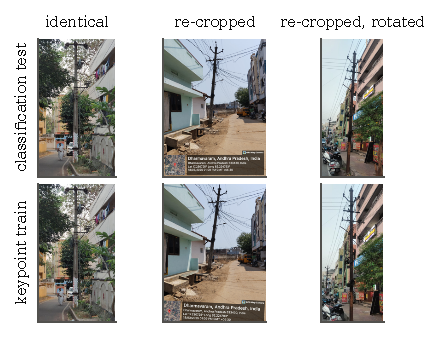
\includegraphics[width=0.5\linewidth]{leakage_examples}
  \caption{Examples of cross-task leakage. Top: classification test split; bottom: keypoint training split.}
  \label{fig:leakage}
\end{figure}

In this work, keypoint labels are used \emph{only} for classification-training images whose file stem and image size match
a keypoint image (1149 of the 1426 Leaned / Straight training images; 87 size mismatches are dropped). The
keypoint loss is masked for Rejected images and for images without a match. Validation and test keypoints are
never used for training or model selection; they are used only for evaluation in \cref{sec:labels,sec:xai}.
Augmentation is restricted to horizontal flips and colour jitter, which do not change the lean label;
rotations and shears are excluded because they would.

\subsection{What do the labels encode?}
\label{sec:labels}
For images with keypoints we compute the ground-truth (GT) axis angle from vertical in pixel space,
$\theta = \operatorname{atan2}(|x_t - x_b|\,W,\; |y_t - y_b|\,H)$, where $(x_b, y_b)$ and $(x_t, y_t)$ are the
normalised bottom and top keypoints and $W \times H$ is the image size.

\Cref{fig:anglehist} shows the distribution of $\theta$ by class for the 1149 training images with keypoints
(757 Straight, 392 Leaned; angles above $20^\circ$ are collected in the last bin). No Straight pole has
$\theta > 10^\circ$, but 16.8\% of Leaned poles have $\theta < 3^\circ$. The median angle is $6.1^\circ$ for
Leaned and $1.0^\circ$ for Straight. A single threshold fitted on training data, $3.03^\circ$, reproduces the
binary label for 90.9\% of training, 93.1\% of validation and 91.6\% of test images with keypoints. The
$10^\circ$ rule used by \citet{masabathula2026smartphone} reproduces only 77.6\% of the test labels, even with
GT keypoints. The two thresholds are marked in \cref{fig:anglehist} (solid and dashed). The annotators therefore applied an implicit threshold of about $3^\circ$, with a band of
genuine disagreement around it. Since the GT-angle rule reaches 91.6\% on Leaned vs.\ Straight, this is a
practical upper bound for any image-based model that has to reproduce these labels.

\begin{figure}[t]
  \centering
  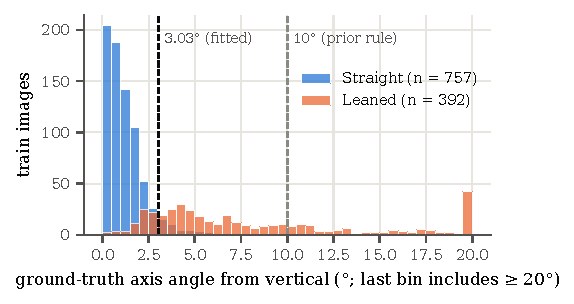
\includegraphics[width=0.6\linewidth]{label_angle_hist}
  \caption{Ground-truth axis angle by class (training images with keypoints).}
  \label{fig:anglehist}
\end{figure}

% =====================================================================================================
\section{Method}
\label{sec:method}

\subsection{Model}
The model (\cref{fig:model}) is a ViT-B/14 backbone, either DINOv2 \citep{oquab2024dinov2} or DINOv2 with
registers \citep{darcet2024registers}, fully fine-tuned at $448 \times 448$ pixels (a $32 \times 32$ grid of
patch tokens). The classification head receives the concatenation of the final CLS token and the mean of the
patch tokens, followed by LayerNorm, dropout (0.2) and a linear layer with three outputs. The keypoint head
uses two learned queries (bottom, top) that attend to the patch tokens through one multi-head
cross-attention layer (8 heads); each output passes through LayerNorm, a two-layer MLP with GELU and a
sigmoid, giving normalised coordinates $(x_b, y_b, x_t, y_t)$. Register tokens are excluded from both heads.

\begin{figure}[t]
\centering
\resizebox{\linewidth}{!}{%
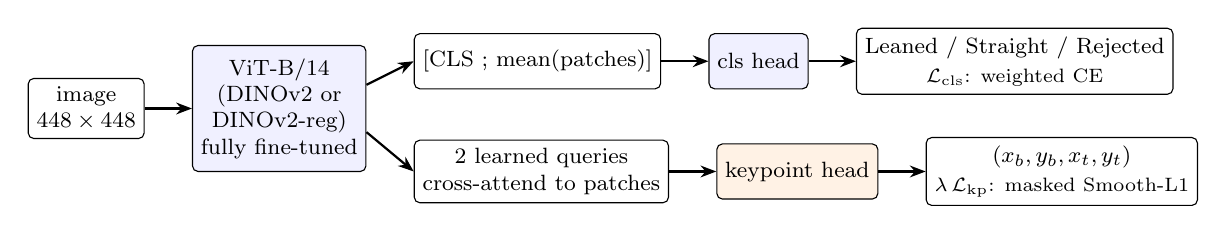
\begin{tikzpicture}[font=\footnotesize, node distance=4mm and 6mm,
  box/.style={draw, rounded corners=2pt, align=center, minimum height=7mm, inner sep=3pt},
  arr/.style={-{Stealth[length=2mm]}, thick}]
  \node[box] (img) {image\\$448\times448$};
  \node[box, right=of img, minimum height=16mm, fill=blue!6] (bb) {ViT-B/14\\(DINOv2 or\\DINOv2-reg)\\fully fine-tuned};
  \node[box, right=of bb, yshift=6mm] (pool) {[CLS ; mean(patches)]};
  \node[box, right=of pool, fill=blue!6] (ch) {cls head};
  \node[box, right=of ch] (cl) {Leaned / Straight / Rejected\\[1pt]{\scriptsize $\mathcal{L}_{\mathrm{cls}}$: weighted CE}};
  \node[box, right=of bb, yshift=-8mm] (xa) {2 learned queries\\cross-attend to patches};
  \node[box, right=of xa, fill=orange!10] (kh) {keypoint head};
  \node[box, right=of kh] (kp) {$(x_b,y_b,x_t,y_t)$\\[1pt]{\scriptsize $\lambda\,\mathcal{L}_{\mathrm{kp}}$: masked Smooth-L1}};
  \draw[arr] (img) -- (bb);
  \draw[arr] (bb.east) ++(0,3mm) -- (pool.west);
  \draw[arr] (pool) -- (ch); \draw[arr] (ch) -- (cl);
  \draw[arr] (bb.east) ++(0,-3mm) -- (xa.west);
  \draw[arr] (xa) -- (kh); \draw[arr] (kh) -- (kp);
\end{tikzpicture}}
\caption{The multi-task network.}
\label{fig:model}
\end{figure}

\subsection{Losses}
The classification loss is the class-weighted cross-entropy with weights inversely proportional to the class
frequencies of the training split. The keypoint loss is a Smooth-L1 loss ($\beta = 0.02$) on the four
normalised coordinates, averaged over the images of the batch that have keypoints:
\begin{equation}
  \mathcal{L} = \mathcal{L}_{\mathrm{cls}} + \lambda \,
  \frac{\sum_i m_i \, \tfrac{1}{4}\sum_{j=1}^{4} \mathrm{SmoothL1}(\hat{k}_{ij} - k_{ij})}{\sum_i m_i},
\end{equation}
where $m_i \in \{0, 1\}$ indicates a valid keypoint label. We call the model trained with
$\mathcal{L}_{\mathrm{cls}}$ only \cls{} (its keypoint head is present but receives no gradient) and the joint
model \mt{}. Two further variants that feed the
predicted axis geometry into the classifier (\texttt{mt\_geo}, with and without gradient through the
keypoints) were evaluated at default settings only and are reported in Appendix~\ref{app:default}.

\subsection{Angle-aware soft targets}
\label{sec:softtargets}
For Leaned and Straight training images with keypoints, the one-hot target $\mathbf{e}_y$ is replaced by
\begin{equation}
  \mathbf{t} = (1-\alpha)\,\mathbf{e}_y + \alpha\,[\,p,\; 1-p,\; 0\,], \qquad
  p = \sigma\!\left(\frac{\theta - \theta_0}{\tau}\right),
  \label{eq:soft}
\end{equation}
where $\theta$ is the GT axis angle and $p$ is a ``lean probability'' implied by the angle. We fixed
$\alpha = 0.5$, $\theta_0 = 3.03^\circ$ (fitted on training data, \cref{sec:labels}) and $\tau = 1^\circ$
before any run; they were not tuned. Because $\alpha = 0.5$, the annotated class always keeps at least half of
the mass: labels are softened, never flipped. Rejected images and images without keypoints keep one-hot
targets. The loss is the class-weighted soft cross-entropy
$-\sum_i \sum_c w_c t_{ic} \log \hat{p}_{ic} / \sum_i \sum_c w_c t_{ic}$, which equals the hard loss for
one-hot targets. On average, the soft targets move 0.089 of the mass off the annotated class (0.099 for
Leaned and 0.084 for Straight).

Two controls use the same images and the same target mass but no per-image angle information. The
shuffled-angle control applies \cref{eq:soft} with the angles randomly permuted among the eligible images of
the same class, which keeps the per-class distribution of targets identical. The uniform-smoothing control moves
the class-wise mean mass (0.099 or 0.084) of every eligible image from its label to the other lean class.

\subsection{Training and model selection}
We use AdamW \citep{loshchilov2019adamw} (weight decay 0.05), separate learning rates for the backbone and the
heads, a one-cycle schedule \citep{smith2019superconvergence} with 10\% warm-up, batch size 16 and mixed
precision. The checkpoint with the best validation Macro-F1 is kept, and the test split is evaluated once per
run.

Both variants receive the same random search \citep{bergstra2012random}: 8 shared configurations of backbone
learning rate, head learning rate and number of epochs (configuration 0 is the default), each trained with two
search seeds. The \mt{} variant additionally receives a loss weight $\lambda \in \{1, 2, 5, 10\}$, with each
value drawn twice, so it gets no extra trials. Selection uses the mean validation Macro-F1; the test split is
not loaded during the search. The selected configuration is then trained with seeds 0--2 and evaluated once on
test. All follow-up experiments reuse the configurations selected for DINOv2 without re-tuning, which is
conservative for the follow-up interventions.

\subsection{Statistics}
The test set has 227 images, so we use paired tests on the same images. For each model, the per-image
prediction is evaluated for every seed, and the metric is averaged over seeds. Differences between two models
are reported with a 95\% paired bootstrap confidence interval (10{,}000 resamples of the test images,
\citealp{efron1993bootstrap}) and an exact McNemar test \citep{mcnemar1947} on the seed-majority-vote
predictions, with Holm correction \citep{holm1979} over the comparisons of each family. We call a difference
significant only if the bootstrap interval excludes zero. The explainability metrics are compared per image
with the bootstrap and a Wilcoxon signed-rank test \citep{wilcoxon1945}. Calibration is measured with the
negative log-likelihood (NLL) and the expected calibration error (ECE, 15 equal-width bins,
\citealp{guo2017calibration}).

\subsection{Pre-specification}
After the main experiments (\cref{sec:main}), each follow-up hypothesis was written to the project repository
before its runs, together with its intervention, primary and secondary outcomes, predicted direction, and,
where relevant, a decision rule. This applies to the experiments on photometric augmentation, reduced training
data, soft targets (including their replication and controls) and explainability. The time-stamped commit
history shows
the order of design and results; the single amendment made after a code check is reported in \cref{sec:xai}.
The main comparison and the diagnostic analyses of \cref{sec:labels,sec:errors} were not pre-specified.

% =====================================================================================================
\section{Results}
\label{sec:results}

\subsection{Main comparison: does keypoint supervision help?}
\label{sec:main}

On DINOv2, both variants select the same configuration (backbone learning rate $10^{-5}$, head learning rate
$3 \times 10^{-4}$, 15 epochs; $\lambda = 2$ for \mt{}), with tied validation Macro-F1 (85.17 vs.\ 85.10).
The \cls{} variant is far more sensitive to hyper-parameters (79.3--85.2 across configurations) and to the
seed: at the default configuration its two search seeds differ by 17 points (70.9 vs.\ 88.0). The \mt{}
variant stays within 81.8--85.1. On DINOv2 with registers, \cls{} selects the default configuration and \mt{}
a configuration with $\lambda = 1$ and 25 epochs; all configurations lie within 81.6--84.6 for both variants.

\Cref{tab:main} shows the tuned models (mean $\pm$ standard deviation over seeds 0--2; the last column is
the Macro-F1 of the seed-majority vote, and the lower part gives the \mt{} $-$ \cls{} difference with its paired
bootstrap 95\% confidence interval and the Holm-adjusted McNemar $p$). Keypoint supervision changes Macro-F1 by $+1.23$ points on DINOv2 and
by $-1.34$ points on DINOv2 with registers; both confidence intervals contain zero (\cref{fig:forest}). At
default settings, before tuning, the same comparison gave $+4.63$ [$+1.98, +7.46$] and $-3.71$
[$-6.61, -0.99$] (Appendix~\ref{app:default}), so the apparently large effects were caused by untuned
hyper-parameters, not by the auxiliary task. \Cref{fig:forest} summarises all effects of this study on
test Macro-F1; its four groups correspond, from top to bottom, to this section and to
\cref{sec:h1,sec:h3,sec:h2}. Only the comparison of soft targets with uniform smoothing has an interval above
zero, and it is not significant under McNemar with Holm correction.

Run-to-run variation is of the same size as these effects. For DINOv2 with registers, the search selected the
default configuration for \cls{}, so the final runs repeated exactly an earlier training setting with the same
seeds. Non-deterministic GPU kernels alone changed the test Macro-F1 by $-1.06$ points on average
($+1.9$, $-2.6$, $-2.5$ per seed).

After tuning, DINOv2 is the better backbone ($-4.76$ [$-7.98, -1.94$] Macro-F1 for \mt{} with registers;
$-2.19$ [$-5.48, +1.09$] for \cls{}). All tuned models lie within the 95\% confidence interval of the DINOv3
baseline reported on the dataset card (84.14 accuracy, 81.74 Macro-F1), which we could not reproduce because
the DINOv3 weights are gated. We make no claim of outperforming it.

\begin{table}[t]
\centering
\caption{Tuned models on the test split.}
\label{tab:main}
\small
\resizebox{\linewidth}{!}{%
\begin{tabular}{llcccccc}
\toprule
backbone & model & Acc. & Macro-F1 & F1$_\mathrm{L}$ & F1$_\mathrm{S}$ & F1$_\mathrm{R}$ & vote \\
\midrule
\multirow{2}{*}{DINOv2}     & \cls{} & 86.34 $\pm$ 0.76 & 83.50 $\pm$ 0.67 & 78.8 & 91.3 & 80.4 & 83.30 \\
                            & \mt{}  & 86.93 $\pm$ 2.17 & 84.72 $\pm$ 2.29 & 81.5 & 91.2 & 81.4 & 87.37 \\
\multirow{2}{*}{DINOv2-reg} & \cls{} & 83.99 $\pm$ 2.22 & 81.31 $\pm$ 2.64 & 77.9 & 89.1 & 76.9 & 81.47 \\
                            & \mt{}  & 83.26 $\pm$ 0.88 & 79.97 $\pm$ 0.97 & 75.6 & 89.2 & 75.1 & 83.60 \\
\midrule
DINOv3 (card)$^\dagger$     & --     & 84.14 & 81.74 & -- & -- & -- & -- \\
\bottomrule
\end{tabular}}

\vspace{2mm}
\begin{tabular}{lcc}
\toprule
comparison & $\Delta$ Macro-F1 [95\% CI] & McNemar $p$ (Holm) \\
\midrule
DINOv2: \mt{} $-$ \cls{}     & $+1.23$ [$-2.01, +4.70$] & 0.24 (0.29) \\
DINOv2-reg: \mt{} $-$ \cls{} & $-1.34$ [$-3.93, +1.15$] & 0.24 (0.71) \\
\bottomrule
\end{tabular}

\vspace{1mm}
\footnotesize $^\dagger$Reported on the dataset card.
\end{table}

\begin{figure}[t]
  \centering
  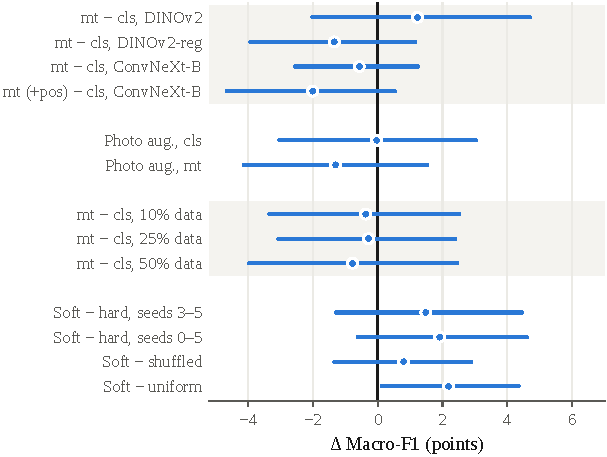
\includegraphics[width=0.62\linewidth]{effects_forest}
  \caption{Effects on test Macro-F1 with paired bootstrap 95\% confidence intervals.}
  \label{fig:forest}
\end{figure}

\subsection{Where do the errors come from?}
\label{sec:errors}
\Cref{fig:errangle} breaks the test errors of the tuned DINOv2 models on Leaned / Straight images down by GT
angle (mean over three seeds; the six bins contain 84, 27, 10, 9, 7 and 6 images). Outside
2--$6^\circ$, errors are rare. Inside this band (37 images, shaded in the figure), the tuned models err on 20--28\% of the images, which
is where the labels themselves are inconsistent (\cref{sec:labels}). On Leaned vs.\ Straight, the tuned DINOv2
\mt{} model reaches 90.4\% accuracy, close to the 91.6\% of the GT-angle rule. The remaining headroom for
Macro-F1 therefore lies mainly in the Rejected class (recall 77.5\% for \cls{} and 86.5\% for \mt{}) and in
the ambiguous band. Rejected is heterogeneous: dark images make up 6.8\% of the Rejected training images but
less than 1\% of the other classes, and visual inspection of the errors shows multi-pole scenes and strong
camera tilt as further causes.

The keypoint head of the tuned DINOv2 \mt{} model predicts the axis angle with a mean absolute error of
$0.97^\circ$ (median $0.63^\circ$; correlation 0.95 with the GT angle). A hybrid rule in which the
classifier decides Rejected and the predicted angle decides Leaned vs.\ Straight reaches 68.5 $\pm$ 1.6
Macro-F1 with the $10^\circ$ threshold and 81.9 $\pm$ 3.3 with a threshold selected on validation data
($3.2^\circ \pm 0.3^\circ$), both below the classifier (84.7). The learned classifier is therefore the better
decision rule, but the joint model provides an interpretable angle estimate at no extra cost.

\begin{figure}[t]
  \centering
  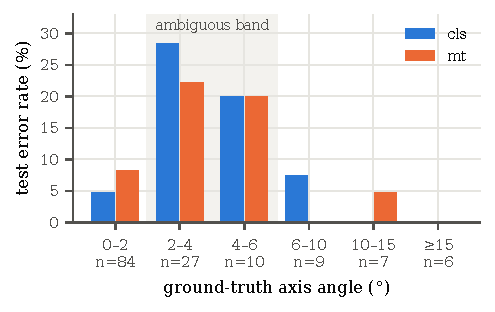
\includegraphics[width=0.6\linewidth]{error_by_angle}
  \caption{Test error rate by ground-truth axis angle.}
  \label{fig:errangle}
\end{figure}

\subsection{Photometric augmentation}
\label{sec:h1}
We hypothesised that the over-representation of dark images in Rejected acts as a shortcut, and that photometric
augmentation (random gamma in $[0.5, 2]$ with $p = 0.5$; low-light simulation by scaling intensities by
0.15--0.5 and adding Gaussian noise, $p = 0.25$) should raise the Rejected F1 and Macro-F1.
The hypothesis is not supported (\cref{tab:h1}, DINOv2, seeds 0--2, differences to the base augmentation
with paired bootstrap 95\% confidence intervals): Macro-F1 does not change, the Rejected F1 does not rise, and the
false-Rejected rate on low-light Leaned / Straight test images (lowest quartile of mean grey value) stays at
7.6\% for \cls{}. The association between darkness and Rejected is therefore not a simple intensity
shortcut: low-light images are also blurred, back-lit or noisy, in ways that resemble genuinely unusable
images.

\begin{table}[t]
\centering
\caption{Effect of photometric augmentation. FR-dark: false-Rejected rate on low-light images.}
\label{tab:h1}
\small
\begin{tabular}{lcccc}
\toprule
model & Macro-F1 & $\Delta$ [95\% CI] & F1$_\mathrm{R}$ & FR-dark \\
\midrule
\cls{}, base aug.  & 83.50 $\pm$ 0.67 & --                       & 80.4 & 7.6\% \\
\cls{}, photo aug. & 83.47 $\pm$ 1.72 & $-0.03$ [$-3.03, +3.03$] & 79.0 & 7.6\% \\
\mt{}, base aug.   & 84.72 $\pm$ 2.29 & --                       & 81.4 & 10.4\% \\
\mt{}, photo aug.  & 83.42 $\pm$ 1.22 & $-1.30$ [$-4.12, +1.53$] & 78.9 & 8.3\% \\
\bottomrule
\end{tabular}
\end{table}

\subsection{Training with less data}
\label{sec:h3}
An auxiliary task may matter more when labelled data are scarce, so we predicted that the \mt{} $-$ \cls{}
difference would be positive and grow as the training set shrinks. We trained on stratified 10, 25 and 50\%
subsets of the training split (the same subset for \cls{} and \mt{} of a given seed), keeping the number of
optimisation steps equal to the full-data runs. \Cref{fig:dataeff} shows the mean over three seeds and a band
of $\pm$ one standard deviation for 170, 426, 853 and 1706 training images (log scale). The prediction was
not confirmed. The
learning curve is steep, from 83.5 to 68.8 Macro-F1 for \cls{}, with most of the loss in the Rejected F1 (80
$\rightarrow$ 51), so the design had room to show an effect. Yet the difference stays within one point at every
fraction ($-0.37$ [$-3.34, +2.51$] at 10\%, $-0.28$ [$-3.06, +2.40$] at 25\%, $-0.78$ [$-3.96, +2.45$] at
50\%).

\begin{figure}[t]
  \centering
  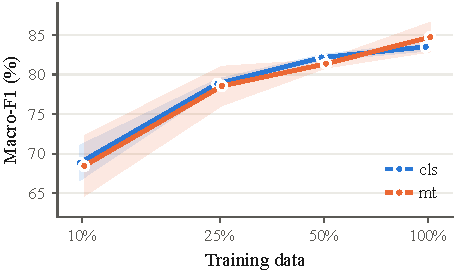
\includegraphics[width=0.6\linewidth]{data_efficiency}
  \caption{Test Macro-F1 against the amount of training data.}
  \label{fig:dataeff}
\end{figure}

\subsection{Angle-aware soft targets}
\label{sec:h2}
We predicted that soft targets from the GT angle (\cref{sec:softtargets}) would raise Macro-F1,
reduce errors in the 2--$6^\circ$ band and improve calibration. On seeds 0--2, every outcome moved in the
predicted direction for \cls{}: Macro-F1 85.84 $\pm$ 1.33 ($+2.34$ [$-1.29, +6.26$]), errors in the band
26.1\% $\rightarrow$ 17.1\%, NLL 0.609 $\rightarrow$ 0.461 and ECE 10.4\% $\rightarrow$ 6.7\%. For \mt{} the
effects were smaller ($+0.44$ [$-2.49, +3.23$]).

Because soft targets also act as label smoothing, we pre-specified a
replication on new seeds (3--5) and the two controls of \cref{sec:softtargets} (seeds 0--5), with the decision
rule that an angle-specific benefit would be claimed only if soft targets beat both controls in Macro-F1 with
a confidence interval above zero. \Cref{tab:h2b} shows the results for \cls{} on DINOv2 over seeds 0--5
(calibration averaged over seeds) and the Macro-F1 differences with paired bootstrap 95\% confidence
intervals. The gain keeps its sign on the new seeds
but shrinks to $+1.49$ [$-1.28, +4.44$]. Soft targets do not beat the shuffled-angle control ($+0.80$
[$-1.33, +2.89$]), so the decision rule is not met, and the drop in band errors does not replicate on seeds
3--5 (23.4\% $\rightarrow$ 27.0\%). The calibration gain is robust: NLL falls from 0.577 to 0.475 over six
seeds, and from 0.545 to 0.489 on seeds 3--5 alone. However, both controls reach the same NLL and ECE
(\cref{fig:reliability}). The improvement in calibration is therefore a property of softened targets, not of
the angle information. In the reliability diagram (all seeds pooled, eight equal-mass bins), hard targets are
over-confident, with a pooled ECE of 9.3\%, whereas angle-aware soft targets (6.2\%) and uniform smoothing
(5.8\%) lie close to the diagonal. As an exploratory observation, heterogeneous soft targets (GT or shuffled angles)
tend to do better than uniform smoothing of the same mean mass ($+2.19$ [$+0.13, +4.35$] for soft vs.\
uniform), but this is not significant under McNemar with Holm correction.

\begin{table}[t]
\centering
\caption{Soft targets and their controls.}
\label{tab:h2b}
\small
\begin{tabular}{lcccc}
\toprule
targets & Macro-F1 & NLL & ECE & error 2--$6^\circ$ \\
\midrule
hard                                 & 83.18 $\pm$ 1.13 & 0.577 & 10.1\% & 24.8\% \\
soft, GT angle                       & 85.10 $\pm$ 1.98 & 0.475 & 7.5\%  & 22.1\% \\
soft, shuffled angle (control)       & 84.30 $\pm$ 1.66 & 0.476 & 6.4\%  & 20.7\% \\
uniform smoothing (control)  & 82.91 $\pm$ 2.05 & 0.492 & 7.3\% & 24.3\% \\
\bottomrule
\end{tabular}

\vspace{2mm}
\begin{tabular}{lc}
\toprule
comparison & $\Delta$ Macro-F1 [95\% CI] \\
\midrule
soft $-$ hard, new seeds 3--5 (primary)      & $+1.49$ [$-1.28, +4.44$] \\
soft $-$ hard, seeds 0--5                    & $+1.91$ [$-0.61, +4.60$] \\
soft $-$ shuffled-angle control              & $+0.80$ [$-1.33, +2.89$] \\
soft $-$ uniform-smoothing control           & $+2.19$ [$+0.13, +4.35$] \\
\bottomrule
\end{tabular}
\end{table}

\begin{figure}[t]
  \centering
  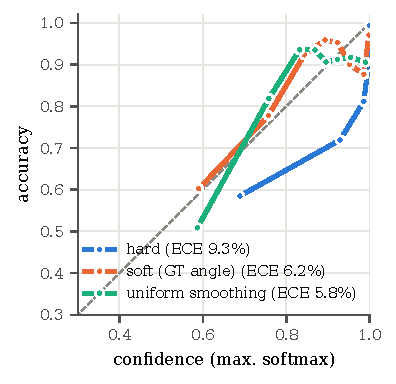
\includegraphics[width=0.46\linewidth]{reliability}
  \caption{Reliability diagram of the \cls{} models on the test split.}
  \label{fig:reliability}
\end{figure}

\subsection{Where does the model look?}
\label{sec:xai}
Even without an accuracy gain, keypoint supervision might make the classifier rely more on the pole than
classification-only training does. We examined this in two pre-specified steps on the 143 Leaned / Straight
test images that have a GT pole box, using the 18 checkpoints of the tuned DINOv2 and DINOv2-with-registers
models and of the soft-target models.

The first step used saliency maps. We computed Grad-CAM at the input of the last transformer block (ReLU of the
gradient-weighted activations of the predicted class, per patch token) and the last-layer attention of the
CLS token, averaged over heads, and measured the share of each map inside the GT box (``energy-in-box''); the
chance level is the box's share of the image, 9.1\% on average. One amendment was made before the full run: a
code check on four images showed hot spots on a few high-norm background tokens, the artifact tokens described
by \citet{darcet2024registers}, so we added a variant that excludes tokens whose pre-LayerNorm norm exceeds three
times the median. The primary metric, Grad-CAM energy-in-box, did not support the hypothesis: it is slightly
\emph{lower} for DINOv2 \mt{} than for \cls{} ($-1.49$ [$-2.10, -0.92$] points, Wilcoxon $p < 0.001$) and
unchanged for DINOv2 with registers ($+0.06$ [$-1.18, +1.27$]). The CLS attention gives the same picture
(\cref{tab:xai}, means over seeds 0--2; ``no art.'': artifact tokens removed; pointing: share of images whose
attention peak lies in the box). The attention concentrates on the pole for all models, with 38--55\% of the
mass in a box that covers 9\% of the image, whereas the last-block Grad-CAM is at chance level and its peak
falls inside the box in only 1--13\% of the images. DINOv2 shows 6--10 artifact tokens per image and DINOv2 with
registers none, and the attention peak lies on the pole in 86--88\% of the images for DINOv2 with registers
against 26--49\% for DINOv2.

\begin{table}[!htb]
\centering
\caption{Relevance inside the ground-truth pole box (chance level 9.1\%).}
\label{tab:xai}
\small
\resizebox{\linewidth}{!}{%
\begin{tabular}{lccccc}
\toprule
model & Grad-CAM & attention & attention, no art. & pointing & artifact tokens \\
\midrule
DINOv2 \cls{}        & 9.8\%  & 41.1\% & 50.8\% & 37.8\% & 7.5 \\
DINOv2 \mt{}         & 8.3\%  & 37.7\% & 49.7\% & 25.6\% & 5.8 \\
DINOv2 soft \cls{}   & 8.1\%  & 41.9\% & 52.1\% & 48.7\% & 9.5 \\
DINOv2-reg \cls{}    & 10.9\% & 54.9\% & 54.9\% & 87.6\% & 0 \\
DINOv2-reg \mt{}     & 10.9\% & 54.7\% & 54.7\% & 85.5\% & 0 \\
\bottomrule
\end{tabular}}
\end{table}

Saliency maps are correlational and can be insensitive to the model \citep{adebayo2018sanity}, so the second
step asked directly whether the decision depends on the pole. We replaced the pole box by a strongly blurred
version of the image (Gaussian, radius 24 pixels at $448 \times 448$) and measured the drop in log-probability
of the originally predicted class; the same was done for five boxes of the same size placed at random without
overlap with the pole. \emph{Pole reliance} is the drop for the pole minus the mean drop for the random boxes.
For 137 of the 143 images, five such boxes could be placed; the other six, with very large poles, were excluded
from this metric as specified in advance. \Cref{tab:occlusion} shows the result, with means over seeds 0--2 and
accuracy computed on these 143 images.

\begin{table}[!htb]
\centering
\caption{Occlusion test.}
\label{tab:occlusion}
\small
\begin{tabular}{lccccc}
\toprule
 & & \multicolumn{2}{c}{prediction flips when blurred} & \multicolumn{2}{c}{accuracy} \\
\cmidrule(lr){3-4}\cmidrule(lr){5-6}
model & pole reliance & pole & random box & intact & pole only \\
\midrule
DINOv2 \cls{}       & 1.87 & 49.2\% & 1.8\% & 90.0\% & 49.9\% \\
DINOv2 \mt{}        & 2.01 & 49.4\% & 3.2\% & 89.3\% & 43.8\% \\
DINOv2 soft \cls{}  & 1.64 & 52.0\% & 2.1\% & 91.4\% & 47.3\% \\
DINOv2 soft \mt{}   & 1.71 & 51.7\% & 2.4\% & 89.7\% & 49.4\% \\
DINOv2-reg \cls{}   & 2.26 & 49.4\% & 2.1\% & 88.1\% & 53.4\% \\
DINOv2-reg \mt{}    & 2.58 & 45.9\% & 1.8\% & 87.9\% & 55.0\% \\
\bottomrule
\end{tabular}
\end{table}

All models depend strongly and causally on the pole: blurring it flips about half of the predictions, while
blurring a random region of the same size flips 2--3\%. The pre-specified comparison of \mt{} with \cls{} (paired
over images, Holm over the two backbones) shows a higher pole reliance for \mt{} on DINOv2 with registers
($+0.33$ [$+0.08, +0.58$], Wilcoxon $p = 0.003$, Holm $p = 0.005$) and a smaller, non-significant increase on
DINOv2 ($+0.14$ [$-0.04, +0.32$], $p = 0.32$), so the prediction is only partly supported. Among the secondary
comparisons, soft targets \emph{reduce} pole reliance ($-0.30$ [$-0.49, -0.11$] for \mt{}, Holm $p = 0.002$;
$-0.23$ [$-0.42, -0.04$] for \cls{}, Holm $p = 0.08$), consistent with less confident decisions. DINOv2 with
registers tends to rely more on the pole than DINOv2 ($+0.38$ for \cls{} and $+0.57$ for \mt{}, bootstrap
intervals above zero), but these differences are not significant after Holm correction. Keeping \emph{only} the
pole and blurring everything else reduces accuracy from about 89\% to 44--55\%, so the surroundings matter as
well. A plausible reason is that buildings and the horizon supply a vertical reference for judging lean, although
heavy blurring also moves the images away from the training distribution.

Finally, we compared the attribution methods themselves (\cref{tab:attribution}). Faithfulness was measured by
a deletion test: patches are blurred in the order given by each map, in ten steps up to half of the image, and
the mean drop in log-probability of the predicted class is compared with a random order (all models pooled,
paired over images). A sanity check re-initialised the classification head and the last four blocks of one
model and correlated the maps before and after (median Spearman correlation; a high value means that the map
hardly depends on the trained weights). The gradient-weighted relevance of \citet{chefer2021transformer} is the
most faithful method, closely followed by the CLS attention; attention rollout \citep{abnar2020attention} is
less faithful and fails the sanity check, and the last-block Grad-CAM is barely better than a random order.
CLS attention is the only method that is both faithful and clearly sensitive to the model. Following the
pre-specified rule, \cref{fig:xai} shows the maps of the most faithful method for the first four images of a
pre-specified random sample (seed-0 models; green: GT pole box). For all three models the relevance lies along the pole shaft, and it
is more concentrated for DINOv2 with registers.

\begin{table}[!htb]
\centering
\caption{Comparison of attribution methods.}
\label{tab:attribution}
\small
\begin{tabular}{lccc}
\toprule
method & energy-in-box & deletion gain [95\% CI] & sanity \\
\midrule
Grad-CAM (last block)                     & 8--11\%  & $+0.29$ [$+0.22, +0.37$] & 0.08 \\
attention rollout                         & 10--11\% & $+2.44$ [$+2.15, +2.73$] & 0.96 \\
CLS attention (last layer)                & 38--55\% & $+4.66$ [$+4.35, +4.97$] & 0.03 \\
\citet{chefer2021transformer}             & 35--49\% & $+5.80$ [$+5.50, +6.08$] & 0.70 \\
\bottomrule
\end{tabular}
\end{table}

\begin{figure}[!htb]
  \centering
  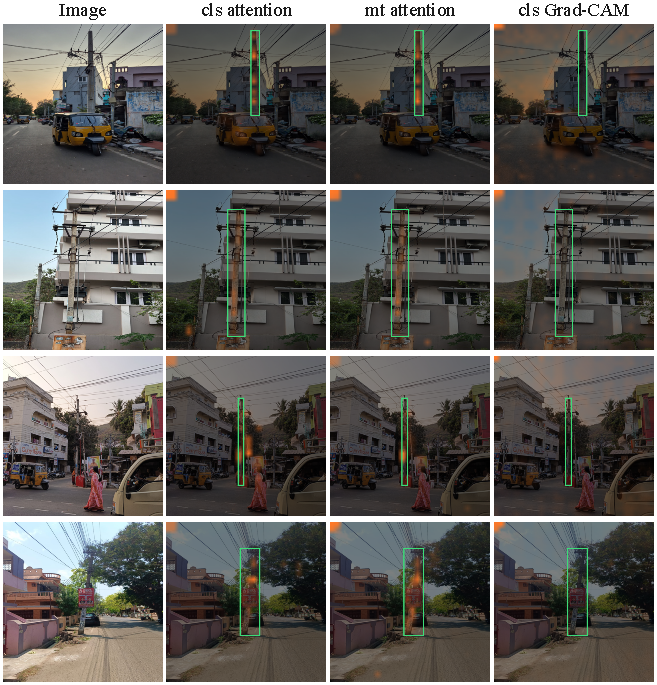
\includegraphics[width=\linewidth]{xai_examples}
  \caption{Relevance maps of the most faithful attribution method for four randomly drawn test images.}
  \label{fig:xai}
\end{figure}

% =====================================================================================================
\section{Discussion}
\label{sec:discussion}

Across four controlled interventions (tuning-matched keypoint supervision, augmentation, reduced data and soft targets), no change to the model or its training raised classification quality
beyond run-to-run noise. The label analysis explains why: on Leaned vs.\ Straight the models are within about
one point of what a perfect angle measurement achieves under the annotators' implicit $3^\circ$ threshold, and
most of the remaining errors are on poles whose label is genuinely ambiguous. Further gains will come from the
labels rather than from the models: an explicit lean criterion (for example a measured angle with a stated
threshold), a clearer definition of Rejected, or graded labels.

Keypoint supervision did not improve classification, but it did not hurt it either, and it makes the model
output the pole axis with sub-degree accuracy. In an inspection tool, this angle is a direct and auditable
explanation of the decision and can be compared with a utility's own tolerance.

Calibration matters in practice. Softened targets reduced the test NLL by about 18\% and the ECE by a quarter. A better calibrated model can be
used with a confidence threshold that sends uncertain images, typically those in the ambiguous band, to a
human inspector. The controls show that simple label smoothing achieves the same benefit, so practitioners
do not need angle annotations for this purpose.

The explainability analyses give a more nuanced picture than the accuracy results alone. All models base their
decision on the pole, as they should, but they also need the surroundings, probably as a vertical reference.
Keypoint supervision made DINOv2 with registers rely more on the pole without making it more accurate, and the
backbone whose attention was most consistently on the pole was the less accurate one. Pole-focused attention
is therefore not a proxy for quality, and saliency maps should not be used to select or justify models for this
task without an accuracy evaluation. The choice of attribution method also matters: the last-block Grad-CAM,
a common default, was barely more informative than a random map for these models.

Finally, the study shows why rigour mattered. Without equal-budget tuning, the first experiments suggested large effects of keypoint supervision ($+4.6$ and
$-3.7$ points) in opposite directions on two backbones. Without replication and controls, the first soft-target experiment would have
suggested an angle-specific gain of $+2.3$ points. Both disappeared under controlled conditions. On test sets
of a few hundred images, single-seed comparisons and untuned baselines are not sufficient.

% =====================================================================================================
\section{Limitations}
\label{sec:limitations}
The study uses a single dataset from one region, and we know of no other public dataset with image-level lean
labels and axis keypoints; the conclusions may not hold for other annotation protocols. With 227 test images,
effects of one to two points cannot be resolved, which our confidence intervals make explicit. We compared two
ViT-B backbones from one family, and DINOv3, used for the dataset-card baseline, could not be evaluated because
its weights are gated. The follow-up experiments reuse hyper-parameters tuned for the baseline, which may
disadvantage the interventions; we accepted this to keep the number of test evaluations small. The
saliency measures are correlational, and the occlusion test replaces regions by a blurred version, which also
moves the images away from the training distribution. Finally,
pre-specification was done in the project's version-controlled repository rather than in a formal registry, and the main comparison
was not pre-specified.

% =====================================================================================================
\section{Conclusion}
\label{sec:conclusion}
We evaluated whether pole-axis keypoints improve image-level lean classification on PD-Defect under
controlled conditions. They do not: after equal-budget tuning, with less data, with stronger augmentation and
with angle-aware targets, the effects stay within the noise of fine-tuning. All models rely on the pole and
on its surroundings, and keypoint supervision increases the reliance on the pole only for one backbone,
without an accuracy gain. The binding constraint is the label, which follows an implicit
$3^\circ$ threshold with an ambiguous band around it. Softened targets improve calibration, but plain
smoothing does the same. We also identified a cross-task leakage in the dataset that affects more than half
of the classification test set for any method that uses the keypoint split, and we describe a leakage-free
protocol for multi-task use of the dataset.

% =====================================================================================================
\section*{Data and code availability}
PD-Defect is available under CC BY 4.0 \citep{pddefect_data}. Code, analysis scripts, all per-run and
per-image results and the pre-specification history are available from the corresponding author on reasonable
request.

\section*{Acknowledgements}
We thank the creators of PD-Defect for releasing the dataset under an open licence. This research received no specific grant from any funding agency in the public,
commercial or not-for-profit sectors.

\section*{Use of AI assistance}
During this study the first author used Claude, an AI assistant developed by Anthropic, as a research
assistant. Under the authors' direction, it searched the literature, wrote and ran the experiment and analysis
code, proposed experimental designs that the authors reviewed and approved before they were run, performed the
statistical analyses, produced the figures and drafted the text of the manuscript. No other AI tool was used.
The authors checked the results and the text and take full responsibility for the content of this article.

\appendix
\renewcommand{\thetable}{\Alph{section}.\arabic{table}}
\section{Results at default hyper-parameters}
\label{app:default}
\Cref{tab:default} reports the test results (mean $\pm$ standard deviation over seeds 0--2) with the default
hyper-parameters: backbone learning rate $2 \times 10^{-5}$, head learning rate $10^{-3}$, 15 epochs and
$\lambda = 5$.

\begin{table}[!ht]
\centering
\caption{Test results at default hyper-parameters.}
\label{tab:default}
\small
\begin{tabular}{llcc}
\toprule
backbone & model & Acc. & Macro-F1 \\
\midrule
DINOv2     & \cls{}                                & 82.23 $\pm$ 2.08 & 78.78 $\pm$ 2.39 \\
DINOv2     & \mt{}                                 & 85.90 $\pm$ 0.44 & 83.41 $\pm$ 0.94 \\
DINOv2     & \texttt{mt\_geo} (predicted geometry)  & 83.55 $\pm$ 1.67 & 80.29 $\pm$ 1.95 \\
DINOv2     & \texttt{mt\_geo\_d} (detached)         & 83.41 $\pm$ 0.67 & 80.38 $\pm$ 1.79 \\
DINOv2-reg & \cls{}                                & 84.88 $\pm$ 1.11 & 82.37 $\pm$ 0.97 \\
DINOv2-reg & \mt{}                                 & 81.50 $\pm$ 1.17 & 78.66 $\pm$ 0.99 \\
\bottomrule
\end{tabular}
\end{table}

At default settings, \mt{} $-$ \cls{} is $+4.63$ [$+1.98, +7.46$] on DINOv2 and $-3.71$ [$-6.61, -0.99$] on
DINOv2 with registers; feeding the predicted geometry to the classifier lowers Macro-F1 ($-3.12$
[$-5.70, -0.73$] for \texttt{mt\_geo} vs.\ \mt{}). These variants were therefore not tuned further.

\section{Hyper-parameter search}
\label{app:search}
\Cref{tab:search} lists the validation Macro-F1 of each configuration (mean over the two search seeds).
Configuration 7 was selected for both variants on DINOv2; on DINOv2 with registers, configuration 0 was
selected for \cls{} and configuration 4 for \mt{}.

\begin{table}[!ht]
\centering
\caption{Validation Macro-F1 of the equal-budget search.}
\label{tab:search}
\small
\begin{tabular}{cccccccc}
\toprule
 & & & & \multicolumn{2}{c}{DINOv2} & \multicolumn{2}{c}{DINOv2-reg} \\
\cmidrule(lr){5-6}\cmidrule(lr){7-8}
cfg & lr backbone & lr head & epochs & \cls{} & \mt{} ($\lambda$) & \cls{} & \mt{} \\
\midrule
0 & $2\times10^{-5}$ & $10^{-3}$          & 15 & 79.47 & 83.43 (5)  & 84.46 & 84.39 \\
1 & $5\times10^{-5}$ & $3\times10^{-4}$   & 15 & 79.33 & 81.78 (10) & 82.20 & 81.92 \\
2 & $3\times10^{-5}$ & $10^{-3}$          & 15 & 81.78 & 82.87 (10) & 83.15 & 83.75 \\
3 & $10^{-5}$        & $10^{-3}$          & 25 & 84.36 & 84.60 (2)  & 83.35 & 84.11 \\
4 & $2\times10^{-5}$ & $3\times10^{-3}$   & 25 & 81.02 & 82.44 (1)  & 83.74 & 84.57 \\
5 & $3\times10^{-5}$ & $3\times10^{-3}$   & 25 & 82.66 & 82.61 (5)  & 83.02 & 81.64 \\
6 & $10^{-5}$        & $3\times10^{-3}$   & 25 & 84.64 & 83.56 (1)  & 83.73 & 83.03 \\
7 & $10^{-5}$        & $3\times10^{-4}$   & 15 & 85.17 & 85.10 (2)  & 83.90 & 83.72 \\
\bottomrule
\end{tabular}
\end{table}

\bibliographystyle{unsrtnat}
\bibliography{references}

\end{document}
